\section{Overview}
\label{sec:overview}
\label{sec:examples}

% RefTypes
% Reflection
% Equational Reasoning
% Proof Search
% Typeclass Laws

We start with an overview of how SMT-based refinement
reflection lets us write proofs as plain
functions and how \pbesym automates equational reasoning.

\subsection{Refinement Types}\label{subsection:overview:refinements}

First, we recall some preliminaries about specification
and verification with refinement types.

\mypara{Refinement types} are the source program's (here
Haskell's) types refined with logical predicates drawn
from an SMT-decidable logic~\citep{ConstableS87,Rushby98}.
%
For example, we define "Nat" as the set of "Integer" values
"v" that satisfy the predicate "0 <= v" from
the quantifier-free logic of linear arithmetic and
uninterpreted functions (QF-UFLIA~\cite{SMTLIB2}):
%
\begin{mcode}
    type Nat = { v:Integer | 0 <= v }
\end{mcode}

\mypara{Specification \& Verification}
%
% We can define and type the textbook Fibonacci function as follows.
Throughout this section,
to demonstrate the proof features we add to \toolname,
we will use the textbook Fibonacci function which we type as follows.
%
\begin{mcode}
    fib :: Nat -> Nat
    fib 0 = 0
    fib 1 = 1
    fib n = fib (n-1) + fib (n-2)
\end{mcode}
%
To ensure termination, the input type's
refinement specifies a \emph{pre-condition}
that the parameter must be "Nat".
The output type's refinement specifies
a \emph{post-condition} that the result
is also a "Nat".
%
Refinement type checking automatically
verifies that if "fib" is invoked with
a non-negative "Integer", then it terminates
and yields a non-negative "Integer".

\mypara{Propositions}
%
We define a data type representing propositions
as an alias for unit:
%
\begin{mcode}
    type $\typp$ = ()
\end{mcode}
%
\VC{Prop is also in HOL, and it's encoded
  as Bool, so this might be confusing,
  maybe this should be Proof instead?}
%
which can be \emph{refined} with propositions about
the code, \eg that $2 + 2$ equals $4$
%
\begin{mcode}
    type Plus_2_2 = { v: $\typp$ | 2 + 2 = 4 }
\end{mcode}
%
For simplicity, in \toolname, we abbreviate the above
to "type Plus_2_2 = { 2 + 2 = 4 }".

\mypara{Universal \& Existential Propositions}
%
Using the standard encoding of~\citet{CHIso},
known as the Curry-Howard isomorphism,
refinements encode universally-quantified propositions as
\emph{dependent function} types of the form:
%
\begin{mcode}
    type Plus_comm = x:Integer -> y:Integer -> { x + y = y + x }
\end{mcode}
%
As "x" and "y" refer to arbitrary inputs,
any inhabitant of the above type is a proof
that "Integer" addition commutes.
%

Refinements encode existential quantification via
\emph{dependent pairs} of the form:
%
\begin{mcode}
    type Int_up = n:Integer -> (m::Integer, {n < m})
\end{mcode}
%
The notation "(m :: t, t')" describes dependent pairs
where the name "m" of the first element can appear
inside refinements of the second element.
%
Thus, "Int_up" states the proposition that for
every integer "n", \emph{there exists}
one that is larger than "n".

%\mypara{Complete Specification}
% Thus,
While quantifiers cannot appear directly
inside the refinements, dependent functions and
pairs allow us to specify quantified propositions.
%
One limitation of this encoding is that quantifiers
cannot exist inside refinement's logical connectives (like $\land$ and $\lor$).
%
In \S~\ref{sec:higher-order}, we describe how to
encode logical connectives using data types,
\eg conjunction as a product and disjunction as
a union, how to specify arbitrary,
quantified propositions
using refinement types, \ie have complete specifications,
and how to verify those propositions using refinement
type checking.

\mypara{Proofs}
%
We \emph{prove} the above propositions by
writing Haskell programs, for example
%
\begin{mcode}
    plus_2_2 :: Plus_2_2        plus_comm :: Plus_comm        int_up :: Int_up
    plus_2_2 = ()               plus_comm = \x y -> ()        int_up = \n -> (n+1,())
\end{mcode}
%
Standard refinement typing reduces the above to
the respective \emph{verification conditions} (VCs)
%
$$ \ttrue \Rightarrow 2 + 2 = 4 \quad \quad \quad
   \forall \ x,\ y\ .\ \ttrue \Rightarrow x + y = y + x \quad \quad \quad
   \forall \ n\ . n < n+1 $$
%
%%\begin{align*}
                      %%2 + 2 & = 4 \\
  %%\forall \ x,\ y\ .\ x + y & = y + x
%%\end{align*}
%
which are easily deemed valid by the SMT solver, allowing us
to prove the respective propositions.

\mypara{Soundness and Lazy Evaluation}
%
Readers familiar with Haskell's lazy 
semantics may be concerned that ``bottom'', 
which inhabits all types, makes our proofs suspect.
%
Fortunately, as described in \citet{Vazou14}, \toolname, 
by default, checks that user defined functions 
provably terminate and are total (\ie return non-bottom values, 
and do not throw any exceptions),
which makes our proofs sound.
%
\toolname checks that each function is terminating using 
a \textit{termination metric} 
\ie a natural number that decreases at each recursive call. 
%
For instance, if we generalize the signature 
of "fib" to "Integers", as shown below, then 
\toolname reports a termination error: 
% Assuming the "fib" is typed as follows
%
\begin{mcode}
    fib :: n:Integer -> Integer
\end{mcode}
%
\toolname generates a type error in the definition of "fib" since in 
the recursive calls "fib (n-1)" and "fib (n-2)"
the arguments "n-1" and "n-2"
cannot be proved to be non-negative and less than "n".
%
Both these proof obligations are satisfied when 
the domain of "fib" is restricted to natural numbers. 
%
\begin{mcode}
    fib :: n:Nat -> Nat / [n]
\end{mcode}
%
The above type signature is explicitly annotated 
with the user specified termination metric "/ [n]"
declaring that "n" is the decreasing natural number. 
% 
\toolname heuristically assumes that the termination metric 
is always the first argument of the function (that can be mapped to natural numbers),
thus, the above explicit termination metric can be omitted. 

Not all Haskell functions terminate. 
%
The "lazy" annotation 
deactivates termination 
checking, \eg for the 
the "diverge" function 
shown below.
%
Haskell terms marked as "lazy" 
could \emph{unsoundly} be used 
as proof terms, much like \coq's 
unsoundness with respect to "Admitted". 
%
For example, the following is 
accepted by \toolname 
%
\begin{mcode}
    lazy diverge 
    diverge :: x:Integer -> { x = 0 }
    diverge x = diverge x 
\end{mcode}


\mypara{Totality Checking}
\toolname further checks that all user-specified functions are totally defined. 
For instance the below definition 
%
\begin{mcode}
    fibPartial 0 = 0 
    fibPartial 1 = 1 
\end{mcode}
generates a totality error. 
%
The above definition is completed, by GHC, 
with an "error" invocation
%
\begin{mcode}
    fibPartial 0 = 0 
    fibPartial 1 = 1 
    fibPartial _ = error "undefined" 
\end{mcode}
%
Thus, to check totality, \toolname simply ascribes the precondition "false" to "error"
%
\begin{mcode}
    error :: { v:String | false } -> a
\end{mcode}
%
Thus, to typecheck "fibPartial", \toolname needs to prove that the call to "error" 
is dead-code, \ie happens under an inconsistent environment. As this check fails, 
\toolname generates a totality error. 
%
As with termination checking,
\toolname provides an \textit{unsound}
error function "unsoundError" with no false precondition.

In the sequel (and in our evaluation) 
we assume that proof terms are generated without 
any unsound uses of "lazy" or "unsafeError".
%
However, note that lazy, diverging functions 
can be soundly verified, and diverging code 
can soundly co-exist with terminating proof 
terms: we refer the reader to \citet{Vazou14} for details.

\subsection{Refinement Reflection}\label{subsec:overview:reflection}

Suppose we wish to prove properties about the "fib"
function, \eg that "{fib 2 = 1}".
%
Standard refinement type checking runs into two problems.
%
First, for decidability and soundness, arbitrary
user-defined functions cannot belong in the refinement
logic, \ie we cannot {refer} to "fib" in a refinement.
%
Second, the only specification that a refinement type checker
has about "fib" is its type "Nat -> Nat" which is
too weak to verify "{fib 2 = 1}".
%
To address both problems, we "reflect fib" into the
logic which sets the three steps of refinement
reflection in motion.



\mypara{Step 1: Definition}
%
The annotation creates an \emph{uninterpreted function}
"!fib! :: Integer -> Integer" in the refinement logic.
%
By uninterpreted, we mean that the logical "!fib!"
is not connected to the program function
"fib"; in the logic, "!fib!" only satisfies the
\emph{congruence axiom}
%
$\forall n, m.\ n = m\ \Rightarrow\ \fib{n} = \fib{m}$.
%
On its own, the uninterpreted function is
not terribly useful: we cannot check "{!fib! 2 = 1}"
as the SMT solver cannot prove the
VC 
$\ttrue \Rightarrow \fib{2} = 1$ 
which requires reasoning about "fib"'s
definition.

\mypara{Step 2: Reflection}
%
In the next key step, we reflect the \emph{definition}
of "fib" into its refinement type by automatically
strengthening the user defined type for "fib" to:
%
\begin{mcode}
    fib :: n:Nat -> { v:Nat | v = !fib! n && fibP n }
\end{mcode}
%
where "fibP" is an alias for a refinement
\emph{automatically derived} from the
function's definition:
%
\begin{mcode}
    fibP n $\doteq$ n == 0 $\Rightarrow$ !fib! n = 0
           $\wedge$ n == 1 $\Rightarrow$ !fib! n = 1
           $\wedge$ n  > 1 $\Rightarrow$ !fib n! = !fib! (n-1) + !fib! (n-2)
\end{mcode}

\mypara{Step 3: Application}
%
With the reflected refinement
type, each application of "fib"
in the code automatically
\emph{unfolds} the definition
of "fib" \textit{once} in the logic.
%
We prove "{!fib! 2 = 1}" by:
%
\begin{mcode}
    pf_fib2 :: { !fib! 2 = 1 }
    pf_fib2 = let { t0 = #fib# 0; t1 = #fib# 1; t2 = #fib# 2 } in ()
\end{mcode}
%
We write in bold red, "#f#", to highlight places where the
unfolding of "f"'s definition is important.
%
Via refinement typing, the above yields the
following VC that is discharged by SMT, even
though "!fib!" is uninterpreted:
%
$$(\fibdef\ 0 \ \wedge\ \fibdef\ 1 \ \wedge\ \fibdef\ 2) \  \Rightarrow\ (\fib{2} = 1)$$
%
% \begin{align*}
   % & (\fibdef\ (\fib\ 0)\ 0) \ \wedge\ (\fibdef\ (\fib\ 1)\ 1) \ \wedge\ \\
   % & (\fibdef\ (\fib\ 2)\ 2) \  \Rightarrow\ (\fib{2} = 1)
% \end{align*}
%
The verification of "pf_fib2" relies
merely on the fact that "fib" is applied
to (\ie unfolded at) "0", "1", and "2".
%
The SMT solver automatically \emph{combines}
the facts, once they are in the antecedent.
Thus, the following is also verified:
%
\begin{mcode}
    pf_fib2' :: {v:[Nat] | !fib! 2 = 1 }
    pf_fib2' = [ #fib# 0, #fib# 1, #fib# 2 ]
\end{mcode}

In the next subsection, we will continue to use explicit,
step-by-step proofs as above, but we will introduce tools 
for proof composition.  
%
Then, in \S~\ref{sec:overview:pbe} we will show how to 
eliminate unnecessary details from such proofs, using 
\emph{Proof by Logical Evaluation} (\pbesym).

%% \RN{Is this updated?  I thought we didn't want to show the old/embarrassing fib
%%   proofs?  Or, at least that we would forward reference the PBE stuff?}

\subsection{Equational Proofs}\label{subsection:overview:equational}

We can {structure} proofs to follow the
style of \emph{calculational} or \emph{equational}
reasoning popularized in classic texts~\cite{Dijkstra76,Bird89}
and implemented in \agda~\citep{agdaequational}
and \dafny~\citep{LeinoPolikarpova16}.
%
To this end, we have developed a library
of proof combinators that permits reasoning
about equalities and linear arithmetic.



\mypara{``Equation'' Combinators}
%
We equip \toolname with a family of
equation combinators, "op", for
logical operators in the theory QF-UFLIA,
"op" $\in \{ =, \not =, \leq, <, \geq, > \}$.
%
In Haskell code, to avoid collisions with existing operators,
we further append a colon ``":"'' to these operators, so that ``$=$''
becomes the Haskell operator "(=:)".
%
The refinement type of "op"  \emph{requires}
that $x \odot y$ holds and then \emph{ensures}
that the returned value is equal to "x".
%
For example, we define "(=:)" as:
%
\begin{mcode}
    (=:) :: x:a -> y:{ a | x = y } -> { v:a | v = x }
    x =: _ = x
\end{mcode}
%
and use it to write the following equational proof:
%
\begin{mcode}
    fib2_1 :: { !fib! 2 = 1 }
    fib2_1 =  #fib# 2 =: #fib# 1 + #fib# 0 =: 1 ** QED
\end{mcode} %$
%
where "** QED" constructs proof terms by
casting expressions to \typp in a post-fix
fashion.
\begin{mcode}
    data $\tqed$ = QED            (**) :: a -> $\tqed$ -> $\typp$
                              _ ** QED = ()
\end{mcode}

\mypara{Proof Arguments}
Often, we need to compose lemmas into larger
theorems. For example, to prove "!fib! 3 = 2" we
may wish to reuse "fib2_1" as a lemma.
%
We do so by defining a variant of "(=:)", written as "(=?)",
that takes an explicit proof argument: 
\begin{mcode}
    (=?) :: x:a -> y:a -> { $\typp$ | x = y } -> { v:a | v = x }
    x =? _ _ = x
\end{mcode}
%
We use the "(=?)" combinator to prove that "!fib! 3 = 2".
%
\begin{mcode}
    fib3_2 :: { !fib! 3 = 2 }
    fib3_2 = (#fib# 3 =: fib 2 + #fib# 1 =? 2 dollar fib2_1) ** QED
\end{mcode}
%
Here "fib 2" is not important to unfold, because "fib2_1"
already provides the same information.

\mypara{``Because'' Combinators}
Observe that the proof term "fib3_2" needs parentheses, 
since Haskell's "(dollar)" operator has the lowest (\ie 0) precedence. 
% 
To omit parentheses in proof terms, we define
a ``because'' combinator that operates exactly like Haskell's 
"(dollar)" operator, but has the same precedence as the proof combinators 
"(=:)" and "(=?)".
%
\begin{mcode}
    ($\because$) :: ($\typp$ -> a) -> $\typp$ -> a
    f $\because$ y = f y
\end{mcode}
%
We use the ``because'' combinator to remove the parentheses from the proof term 
"fib3_2".
%
\begin{mcode}
    fib3_2 :: { !fib! 3 = 2 }
    fib3_2 = #fib# 3 =: fib 2 + #fib# 1 =? 2 $\because$ fib2_1 ** QED
\end{mcode}

\mypara{Optional Proof Arguments}
%
Finally, we unify both combinators "(=:)" and "(=?)"
using type classes to define the class method "(=.)" 
that takes an \textit{optional} proof argument, and 
generalize such definitions for each operator in "op". 
%
We define the class "OptEq" to have one method "(=.)" 
that takes two arguments of type "a", to be compared 
for equality, and returns a value of type "r". 
%
\begin{mcode}
    class OptEq a r where
      (=.) :: a -> a -> r
\end{mcode}
%
When instantiating the result type to be the same as the argument type "a", 
"(=.)" behaves as "(=:)".
\begin{mcode}
    instance (a~b) => OptEq a b where
      (=.) :: x:a -> { y:a | x = y } -> { v:b | v = x }
\end{mcode}
%
When the result type is instantiated to be 
a function that given a proof term "$\typp$"
returns the argument type "a", 
"(=.)" behaves exactly as "(=?)".
%
\begin{mcode}
    instance (a~b) => OptEq a ($\typp$ -> b) where
      (=.) :: x:a -> y:a -> { $\typp$ | x = y } -> { v:a | v = x }
\end{mcode}

Thus, "(=.)" takes two arguments to be compared for equality
and, optionally, a proof term argument. 
%
With this, the proof term "fib3_2" is simplified to  
%
\begin{mcode}
    fib3_2 :: { !fib! 3 = 2 }
    fib3_2 = #fib# 3 =. fib 2 + #fib# 1 =. 2 $\because$ fib2_1 ** QED
\end{mcode}

\mypara{Arithmetic and Ordering}
%
Next, lets see how we can use arithmetic and ordering to
prove that "fib" is (locally) increasing, \ie for all $n$,
$\fib{n} \leq \fib{(n+1)}$.
%
\begin{mcode}
    type Up f = n:Nat -> { f n <= f (n + 1) }

    fibUp   :: Up fib
    fibUp 0 =  #fib# 0 $<$. #fib# 1                          ** QED
    fibUp 1 =  #fib# 1 <=. fib 1 + #fib# 0     =. #fib# 2     ** QED
    fibUp n =  #fib# n <=. fib n + #fib# (n-1) =. #fib# (n+1) ** QED
\end{mcode} %$

% \RN{Umm, maybe we could make this a literate document where the code
%   runs? The above looks wrong.  It says that \lstinline{fib n = fib (n+1)} on
%   the last line.}

\mypara{Case Splitting}
%
The proof "fibUp" works by splitting cases on the value of "n".
%
In the cases "0" and "1", we simply assert
the relevant inequalities. These are verified as the
reflected refinement unfolds the definition of
"fib" at those inputs.
%
The derived VCs are (automatically) proved
as the SMT solver concludes $0 < 1$ and $1 + 0 \leq 1$
respectively.
%
When "n" is greater than one, "fib n" is unfolded
to  "fib (n-1) + fib (n-2)", which, as "fib (n-2)"
is non-negative, completes the proof.

\mypara{Induction \& Higher Order Reasoning}
%
Refinement reflection smoothly accommodates induction
and higher-order reasoning.
%
For example, let's prove that every function "f"
that increases locally (\ie "f z <= f (z+1)" for all "z")
also increases globally (\ie "f x <= f y" for all "x < y")
%
%%   fMono :: f:(Nat -> Integer) -> Up f -> x:_ -> y:{x < y} -> {f x <= f y} / [y]
\begin{mcode}
    type Mono = f:(Nat -> Integer) -> Up f -> x:Nat -> y:{ x < y } -> { f x <= f y }

    fMono :: Mono / [y]
    fMono f up x y
      | x+1 == y = f x <=. f (x+1) $\because$ up x <=. f y                          ** QED
      | x+1  < y = f x <=. f (y-1) $\because$ fMono f up x (y-1) <=. f y $\because$ up (y-1) ** QED
\end{mcode}
%
We prove the theorem by induction
on "y" as specified by the
annotation "/ [y]" which states
that "y" is a well-founded
termination metric that decreases
at each recursive call~\citep{Vazou14}.
%
If "x+1 == y", then we call the "up x" proof argument.
%
Otherwise, "x+1 < y", and we use
the induction hypothesis \ie apply
"fMono" at "y-1", after which
transitivity of the less-than
ordering finishes the proof.
%
We can \emph{apply} the general
"fMono" theorem to prove that
"fib" increases monotonically:
%
\begin{mcode}
    fibMono :: n:Nat -> m:{ n < m } -> { !fib! n <= !fib! m }
    fibMono = fMono fib fibUp
\end{mcode}

\subsection{Complete Verification: Automating Equational Reasoning}
\label{sec:overview:pbe}

While equational proofs can be
very \elegant, writing them out
can quickly get exhausting.
%
Lets face it: "fib3_2" is doing
rather a lot of work just to
prove that "fib 3" equals "2"!
%
Happily, the \emph{calculational}
nature of such proofs allows us
to develop the following proof
search algorithm \pbesym that
is inspired by model checking~\cite{CGL92}
%
\begin{itemize}[leftmargin=*]
\item \emphbf{Guard Normal Form:}
%
First, as shown in the definition
of "fibP" in~\S~\ref{subsec:overview:reflection}, each reflected
function is transformed into a
\emph{guard normal form}
%
$\wedge_i (\pred_i \Rightarrow \fapp{\rfun}{x} = \body_i)$
%
\ie a collection of \emph{guards} $\pred_i$
and their corresponding definition $\body_i$.

\item \emphbf{Unfolding:}
Second, given a VC of the form
$\Penv \Rightarrow \pred$,
we iteratively \emph{unfold}
function application terms in
$\Penv$ and $\pred$ by
\emph{instantiating} them with
the definition corresponding to
an \emph{enabled} guard, where
we check enabled-ness by
querying the SMT solver.
%
For example, given the VC
$\ttrue \Rightarrow \fib{3} = 2$,
the guard $3 > 1$ of the application $\fib{3}$ is
trivially enabled,
\ie is true, hence we
strengthen the hypothesis
$\Penv$ with the equality
$\fib{3} = \fib{(3-1)} + \fib{(3-2)}$
corresponding to unfolding the
definition of "fib" at "3".

\item \emphbf{Fixpoint:}
%
We repeat the unfolding process
until either the VC is proved
or we have reached a fixpoint,
\ie no further unfolding is
enabled.
%
For example, the fixpoint
computation of $\fib{3}$ unfolds the definition
of "fib" at "3", "2", "1", and "0"
and then stops as no further
guards are enabled.
\end{itemize}

%% \RN{At this point not sure if this fixpoint iteration is an outer
%%   loop repeating SMT invocation on each iteration.}


\mypara{Automatic Equational Reasoning}
%
In \S~\ref{sec:pbe} we formalize
a notion of \emph{equational proof}
and show that the proof search procedure
\pbesym enjoys two key properties.
%
First, that it is guaranteed to find
an equational proof if one can be constructed 
from unfoldings of function definitions.
(The user must still provide instantiations 
of lemmas and induction hypotheses.) 
%
Second, that under certain conditions readily
met in practice, it is guaranteed to terminate.
%
These two properties allow us to use \pbesym
to predictably automate proofs: the programmer needs
only to supply the relevant induction hypotheses
or helper lemma applications.
%
The remaining long chains of calculations
are performed automatically via SMT-based
\pbesym.
%
That is, the user must provide case statements 
and the recursive structure, but can elide 
the long chains of \lstinline{=.} applications.
%
To wit, with complete proof search,
the proofs of~\S~\ref{subsection:overview:equational} shrink to:
%
\begin{mcode}
    fib3_2 :: {!fib! 3 = 2}       fMono :: Mono / [y]
    fib3_2 = ()                 fMono f up x y    
                                  | x+1 == y = up x
                                  | x+1  < y = up (y-1) &&& fMono up x (y-1)
\end{mcode}
%%%\begin{mcode}
%%%fib3_2 :: {!fib! 3 = 2}   fibUp  :: Up fib   fMono :: Mono / [y]
%%%fib3_2 = ()             fibUp 0 = ()       fMono f up x y
%%%                        fibUp 1 = ()         | x+1 == y = up x
%%%                        fibUp n = ()         | x+1  < y = up (y-1) &&& fMono up x (y-1)
%%%\end{mcode}
%
where the combinator "p &&& q = ()"
inserts the propositions "p" and "q" to the
VC hypothesis.

\mypara{\pbesym vs. Axiomatization}
%
Existing SMT based verifiers like
\dafny~\citep{dafny} and \fstar~\citep{fstar}
use the classical \emph{axiomatic} approach
to verify assertions over user-defined
functions like "fib".
%
In these systems, the function is encoded in the logic
as a universally quantified formula (or axiom):
%
$\forall n.\ \fibdef\ n$
%
after which the SMT solver may
instantiate the above axiom at
"3", "2", "1" and "0" in order to
automatically prove "{fib 3 = 2}".

The automation offered by axioms
is a bit of a devil's bargain,
as axioms render VC checking
\emph{undecidable}, and in
practice automatic axiom
instantiation can easily
lead to infinite ``matching loops''.
%
For example, the existence of
a term \fib{n} in a VC can
trigger the above axiom,
which may then produce
the terms \fib{(n-1)}
and \fib{(n-2)}, which
may then recursively
give rise to further
instantiations
\emph{ad infinitum}.
%
To prevent matching
loops an expert must
carefully craft ``triggers''
or alternatively, provide
a ``fuel'' parameter
that bounds the depth of
instantiation~\citep{Amin2014ComputingWA}.
%
Both these approaches
ensure termination,
but can cause the
axiom to not be
instantiated at
the right places,
thereby rendering
the VC checking
\emph{incomplete}.
%
The incompleteness
is illustrated by
the following example
from the \dafny benchmark
suite~\cite{dafny-github}
%
\begin{mcode}
    pos n | n < 0     = 0                test   :: y:{y > 5} -> {!pos! n = 3 + !pos! (n-3)}
          | otherwise = 1 + pos (n-1)    test _ = ()
\end{mcode}
%% \RN{Ugh, let's make sure the above 2x2 matrix of code doesn't get
%%   page-broken in the final version; its terrible.}
%
\dafny (and \fstar's) fuel-based approach fails
to check the above, when the fuel value is less
than $3$. One could simply raise-the-fuel-and-try-again
but at what point does the user know when to stop?
%
In contrast, \pbesym (1)~does not require any fuel
parameter, (2)~is able to automatically perform
the required unfolding to verify this example,
\emph{and} (3)~is guaranteed to terminate.


\begin{figure}[t!]
\centering
\begin{minipage}[t]{0.45\textwidth}
\begin{mcodef}
app_assoc :: AppendAssoc
app_assoc [] ys zs
  = ([] ++ ys) ++ zs
  =. ys ++ zs
  =. [] ++ (ys ++ zs)         ** QED
app_assoc (x:xs) ys zs
  = ((x : xs) ++  ys)  ++ zs
  =. (x : (xs ++  ys)) ++ zs
  =.  x :((xs ++  ys)  ++ zs)
      $\because$ app_assoc xs ys zs
  =.  x : (xs ++ (ys   ++ zs))
  =. (x : xs) ++ (ys   ++ zs) ** QED
\end{mcodef}
\end{minipage}
\hspace{0.14in}
\begin{minipage}[t]{0.49\textwidth}
\begin{mcodef}
app_assoc             :: AppendAssoc
app_assoc []     ys zs = ()
app_assoc (x:xs) ys zs = app_assoc xs ys zs
\end{mcodef}
\begin{mcodef}
app_right_id          :: AppendNilId
app_right_id []        = ()
app_right_id (x:xs)    = app_right_id xs
\end{mcodef}
\begin{mcodef}
map_fusion            :: MapFusion
map_fusion f g []      = ()
map_fusion f g (x:xs)  = map_fusion f g xs
\end{mcodef}
\end{minipage}
\caption{\textbf{(L)} Equational proof of append associativity. \quad
  \textbf{(R)} \pbesym proof, also of append-id and map-fusion.
%% \RN{Compared to the other code in the document, which has some
%%   color, this totally monochrome figure stands out.  Perhaps we
%%   could turn on some slight colorization of basic punctuation.
%%   Or some targeted formatting of proof combinators.  Listings is
%%   very customizable!}
}
\label{fig:list-laws}
\end{figure}

\subsection{Case Study: Laws for Lists}
\label{sec:overview:lists}

Reflection and \pbesym are not limited to integers.  We end the
overview by showing how they verify textbook properties of lists
equipped with append ("++") and "map" functions:
%
\begin{mcode}
    reflect (++) :: [a] -> [a] -> [a]       reflect map :: (a -> b) -> [a] -> [b]
    []     ++ ys = ys                       map f []     = []
    (x:xs) ++ ys = x : (xs ++ ys)           map f (x:xs) = f x : map f xs
\end{mcode}
%
In \S~\ref{subsec:embedding}
we will describe how the reflection mechanism
illustrated via "fibP" is extended to account for ADTs
using SMT-decidable selection and projection operations,
which reflect the definition of "xs ++ ys" into the refinement as:
%
$\ite{\mathtt{isNil}\ \mathit{xs}}
    {\mathit{ys}}
    {\mathtt{sel1}\ \mathit{xs}\
      \dcons\
      (\mathtt{sel2}\ \mathit{xs} \ \mathtt{++}\  \mathit{ys})}$.
%
% We favor selectors to the axiomatic translation of
% HALO~\citep{HALO} to avoid universally quantified
% formulas and the resulting unpredictability.
%
We require an explicit "reflect" annotation
as not all Haskell functions can be 
reflected into logic, either because it 
is unsound to do so (\eg due to divergence)
or because of limitations of our current 
implementation. 
%
Recall that \toolname verifies that all reflected functions, 
like "(++)" and "map" here, are total~\citep{Vazou14}
and rejects the code otherwise.

\mypara{Laws}
%
We can specify various laws about lists with refinement types.
For example, the below laws state that
%
(1)~appending to the right is an \emph{identity} operation,
%
(2)~appending is an \emph{associative} operation, and
%
(3)~map \emph{distributes} over function composition:
%
\begin{mcode}
    type AppendNilId = xs:_ -> { xs ++ [] = xs }
    type AppendAssoc = xs:_ -> ys:_ -> zs:_ -> { xs ++ (ys ++ zs) = (xs ++ ys) ++ zs }
    type MapFusion   = f:_  -> g:_  -> xs:_ -> { map (f . g) xs = map f (map g xs) }
\end{mcode}

\mypara{Proofs}
%
On the right in Figure~\ref{fig:list-laws}
we show the proofs of these laws using \pbesym,
which should be compared to the classical equational
proof~\eg~by \citet{WadlerCalculating}, shown on the left.
%
With \pbesym, the user need only
provide the high-level structure
--- the case splits and invocations
of the induction hypotheses ---
after which \pbesym automatically
completes the rest of the equational
proof.
%
Thus using SMT-based \pbesym, "app_assoc"
shrinks down to its essence: an induction
over the list "xs".
%
The difference is even more stark with
"map_fusion" whose full equational proof
is omitted, as it is twice as long.

\mypara{\pbesym vs. Normalization}
%
The proofs in Figure~\ref{fig:list-laws}
may remind readers familiar with Type-Theory
based proof assistants (\eg \toolfont{Coq} or
\toolfont{Agda}) of the notions of
\emph{type-level normalization} and
\emph{rewriting} that permit similar
proofs in those systems.
%
While our approach of \pbesym is
inspired by the idea of type
level computation, it differs
from it in two significant ways.
%
First, from a \emph{theoretical} point of view,
SMT logics are not equipped with any notion
of computation, normalization, canonicity
or rewriting.
Instead, our \pbesym algorithm shows how
to \emph{emulate} those ideas by asserting
equalities corresponding to function
definitions (Theorem~\ref{thm:completeness}).
%
Second, from a \emph{practical} perspective,
the combination of (decidable) SMT-based 
theory reasoning and \pbesym's proof search 
can greatly simplify verification.
%
For example, consider the "swap" function
from~\citet{appel-vfa}'s \coq textbook:
%
\begin{mcode}
    swap :: [Integer] -> [Integer]
    swap (x1:x2:xs) = if x1 > x2 then x2:x1:x2 else x1:x2:xs
    swap xs         = xs
\end{mcode}
%
In Figure~\ref{fig:swap} we show four proofs
that "swap" is idempotent:
%
Appel's proof using \coq (simplified by
the use of a hint database and the
arithmetic tactic "omega"), its variant in
\agda (for any Decidable Partial Order),
the \pbesym proof, and 
a proof using the \dafny verifier.
%
It is readily apparent that \pbesym's
proof search, working
hand-in-glove with SMT-based theory
reasoning, makes proving the result
trivial in comparison to \coq or \agda.
%
Of course, proof assistants like
\agda, \coq, and \toolfont{Isabelle}
emit easily checkable certificates
and have decades-worth of tactics,
libraries, and proof scripts that
enable large scale proof engineering.
%
On the other hand, \dafny's fuel-based 
axiom instantiation automatically 
unfolds the definition of "swap" twice, 
thereby completing the proof 
without any user input.
%
These heuristics are 
orthogonal to  \pbesym and can 
be combined with it, if the user 
wishes to trade off predictability 
for even more automation.

% heuristics are compatible with \pbesym, but aren't enabled by default in
% \toolname, \coq, or \agda because they can cause small changes to make proofs fail
% or succeed for seemingly ``magical'' reasons.
%

\begin{figure}[t!]
  \begin{center}
    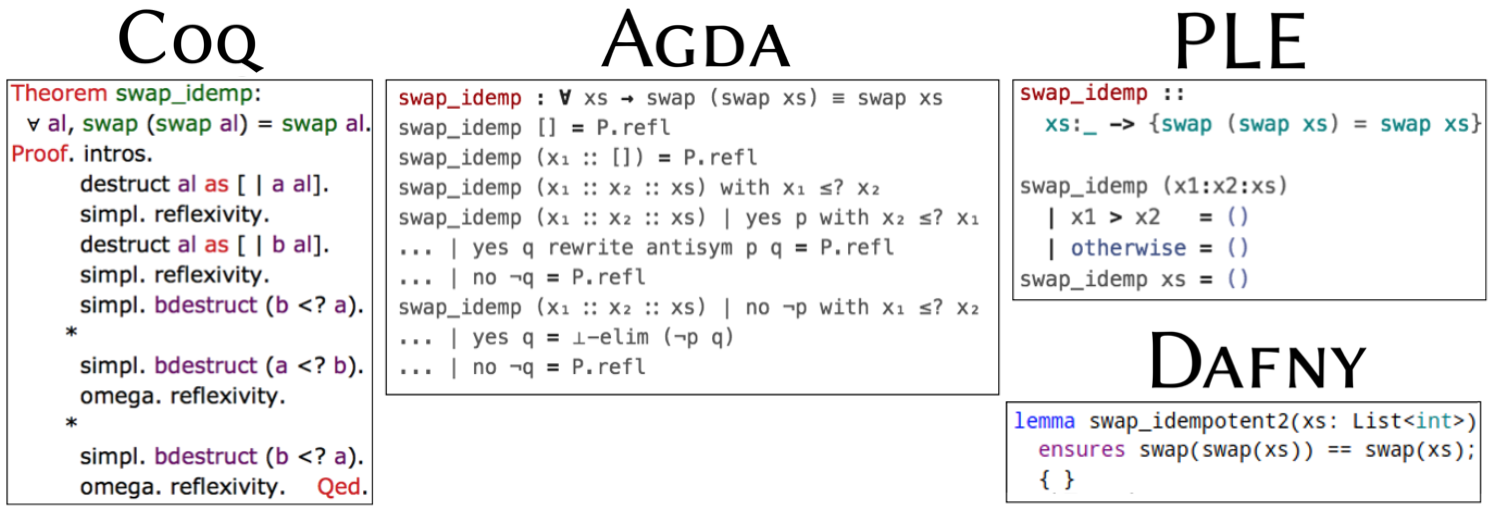
\includegraphics[width=5.5in]{figs/maybe-swap-all-new.png}
  \end{center}
  \vspace{-3mm}
  \caption{Proofs that \texttt{swap} is idempotent with
    \coq, \agda, \dafny and \pbesym.
  }
  \label{fig:swap}
\end{figure}

\mypara{Summary}
%
We saw an overview of an SMT-automated refinement 
type checker that achieves SMT-decidable checking 
by restricting verification conditions to be 
\emph{quantifier-free} and hence, decidable.
%
In existing SMT-based verifiers (\eg \dafny) there 
are two main reasons to introduce quantifiers, namely
%
(1)~to express quantified \emph{specifications} and 
(2)~to encode the semantics of \emph{user-defined functions}.
%
Next, we use propositions-as-types to encode 
quantified specifications and in~\S~\ref{sec:formalism} 
we show how to encode the semantics of user-defined functions 
via refinement reflection.
